%%%%%%%%%%%%%%%%%%%%%%%%%%%%%%%%%%%%%%%%%%%%%%%%%%%%%%%%%%%%%%%%%%%%%%%%%%%%%%%%
%2345678901234567890123456789012345678901234567890123456789012345678901234567890
%        1         2         3         4         5         6         7         8

\documentclass[letterpaper, 10 pt, conference]{ieeeconf}  % Comment this line out if you need a4paper

%\documentclass[a4paper, 10pt, conference]{ieeeconf}      % Use this line for a4 paper

\IEEEoverridecommandlockouts                              % This command is only needed if
                                                          % you want to use the \thanks command

\overrideIEEEmargins                                      % Needed to meet printer requirements.

% See the \addtolength command later in the file to balance the column lengths
% on the last page of the document

% The following packages can be found on http:\\www.ctan.org
\usepackage{graphicx}
\usepackage{hyperref}
\usepackage{textcomp}
%\usepackage{epsfig} % for postscript graphics files
%\usepackage{mathptmx} % assumes new font selection scheme installed
%\usepackage{times} % assumes new font selection scheme installed
%\usepackage{amsmath} % assumes amsmath package installed
%\usepackage{amssymb}  % assumes amsmath package installed

\title{\LARGE \bf
Optimization-based Motion Retargeting Integrating Spatial and Dynamic Constraints
}


\author{Thomas Moulard$^{1}$, Eiichi Yoshida$^{1}$ and Shin'ichiro
  Nakaoka$^{2}$% <-this % stops a space
\thanks{*This work was not supported by any organization}% <-this % stops a space
\thanks{$^{1}$T.~Moulard and E.~Yoshida are with CNRS-AIST JRL (Joint
  Robotics Laboratory), UMI3218/CRT, and $^{1}$S.~Nakaoka are with
  Humanoid Research Group, both National Institute of Advanced Industrial Science and Technology (AIST)
Tsukuba Central 2, 1-1-1 Umezono, Ibaraki 305-8568 Japan
        {\tt\footnotesize \{thomas.moulard, e.yoshida, s.nakaoka\}@aist.go.jp}}%
}


\begin{document}



\maketitle
\thispagestyle{empty}
\pagestyle{empty}


%%%%%%%%%%%%%%%%%%%%%%%%%%%%%%%%%%%%%%%%%%%%%%%%%%%%%%%%%%%%%%%%%%%%%%%%%%%%%%%%
\begin{abstract}
In this paper, we present an optimization-based retargeting method for
precise reproduction of captured human motions by a humanoid robot.
We take into account two important aspects of retargeting
simultaneously: spatial relationship and robot dynamics model.  The
former takes care of the spatial relationship between the body parts
based on ``interaction mesh'' to follow the human motion in a natural
manner, whereas the latter adapts the resulting motion in such a way
that the dynamic constraints such as torque limit or dynamic balance
are being satisfied.  We have integrated the interaction mesh and the
dynamic constraints in an optimization framework, which is
advantageous for generation of natural motions by a humanoid robot
compared to previous work that performs those processes
separately. The re targeted motions are being validated through dynamic
simulations of a humanoid robot.
\end{abstract}


%%%%%%%%%%%%%%%%%%%%%%%%%%%%%%%%%%%%%%%%%%%%%%%%%%%%%%%%%%%%%%%%%%%%%%%%%%%%%%%%
\section{Introduction}
\label{sec:intro}

One of the advantages of human-size humanoid robots is
its ability to generate whole-body motions maintaining similar
dynamics to humans.
This ability allows a humanoid robot to serve as an entertainer like
a dancer of an actor \cite{nakaoka_iros2010}, or also to use various
machines and devices designed for humans \cite{Yokoi03iros}.
As an extension of the latter use, a new application
has recently been studied: a humanoid robot as an evaluator of human
assistive devices \cite{Takanishi06ICRA,Miura13ICRA}.
If a humanoid reproduces human motions faithfully, it can be used to
test the devices instead of human subjects.
This brings several benefits such as no need for ethical
process, repeated test with exactly the same motions under the same
conditions, and qualitative evaluation through sensory measurement
like torque and force.
It has been demonstrated that the human-size humanoid HRP-4C
\cite{Kaneko09Humanoids}  can evaluate the effect of load reduction
quantitatively by estimating motor torque \cite{Miura13ICRA}, taking
an example of a supportive wear called ``Smart Suit Lite''
\cite{Tanaka11JRM} designed to reduce load
at the lower back with embedded elastic bands.

The important issue in those applications is how to generate natural
motions of a humanoid robot.  There have been a number of studies on
``motion retargeting'' techniques in order to generate humanoid
motions based on those of a human measured by a motion capture system.
Retargeting captured motion to humanoids has been actively studied
during the last decade, thanks to the progress of their dynamic
capability. The work of Pollard \cite{Pollard02ICRA} is one of the
pioneering studies that enable reproduction of human motions by a
humanoid, in this case the upper body of Sarcos humanoid robot, by
taking into account various constraints.  Nakaoka et al. developed a
technique to transfer Japanese traditional dancing motions to a
humanoid by introducing a notion of leg task model
\cite{nakaoka_icra2004,nakaoka_2007}.  Miura et al. \cite{Miura11IROS}
devised a walking pattern generator that allows the humanoid robot
HRP-4C to walk in a manner extremely close to humans, including
stretched knees, swing-leg trajectory and single support phase on the
toe.  Other imitation methods have been proposed based on a dynamic
controller \cite{Yamane11humanoids,Ramos11humanoids}, motion
recognition and primitives \cite{Ott08humanoids} and extraction of
upper-body motion from markerless motion input
\cite{Dariush08IROS,Do08humanoids}.


\begin{figure}
\begin{center}
  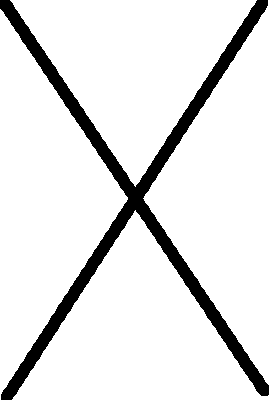
\includegraphics[width=0.6 \linewidth]{figure/fixme.png}
  \label{fig:choreonoid-result}
  \caption{HRP-4C optimized motion using RobOptim and the Choreonoid robotics frameworks.}
\end{center}
\end{figure}

% Human motion based optimization
% Categoraized related work
% Takano
% \begin{itemize}
% \item Pollard (upper body), Dariush, Lee, Kulic, Yamane, Miura, Mansard
%   (walking) Martin Do-KIT
%
% \item Manocha, Kallman: support for humanoid animation -- graphic only
% \item Nakaoka humanoids 2012 -- graphic + robot
% \item Motion optimization Miossec, Suleiman, Lengagne
% \end{itemize}

\begin{figure*}[tb]
  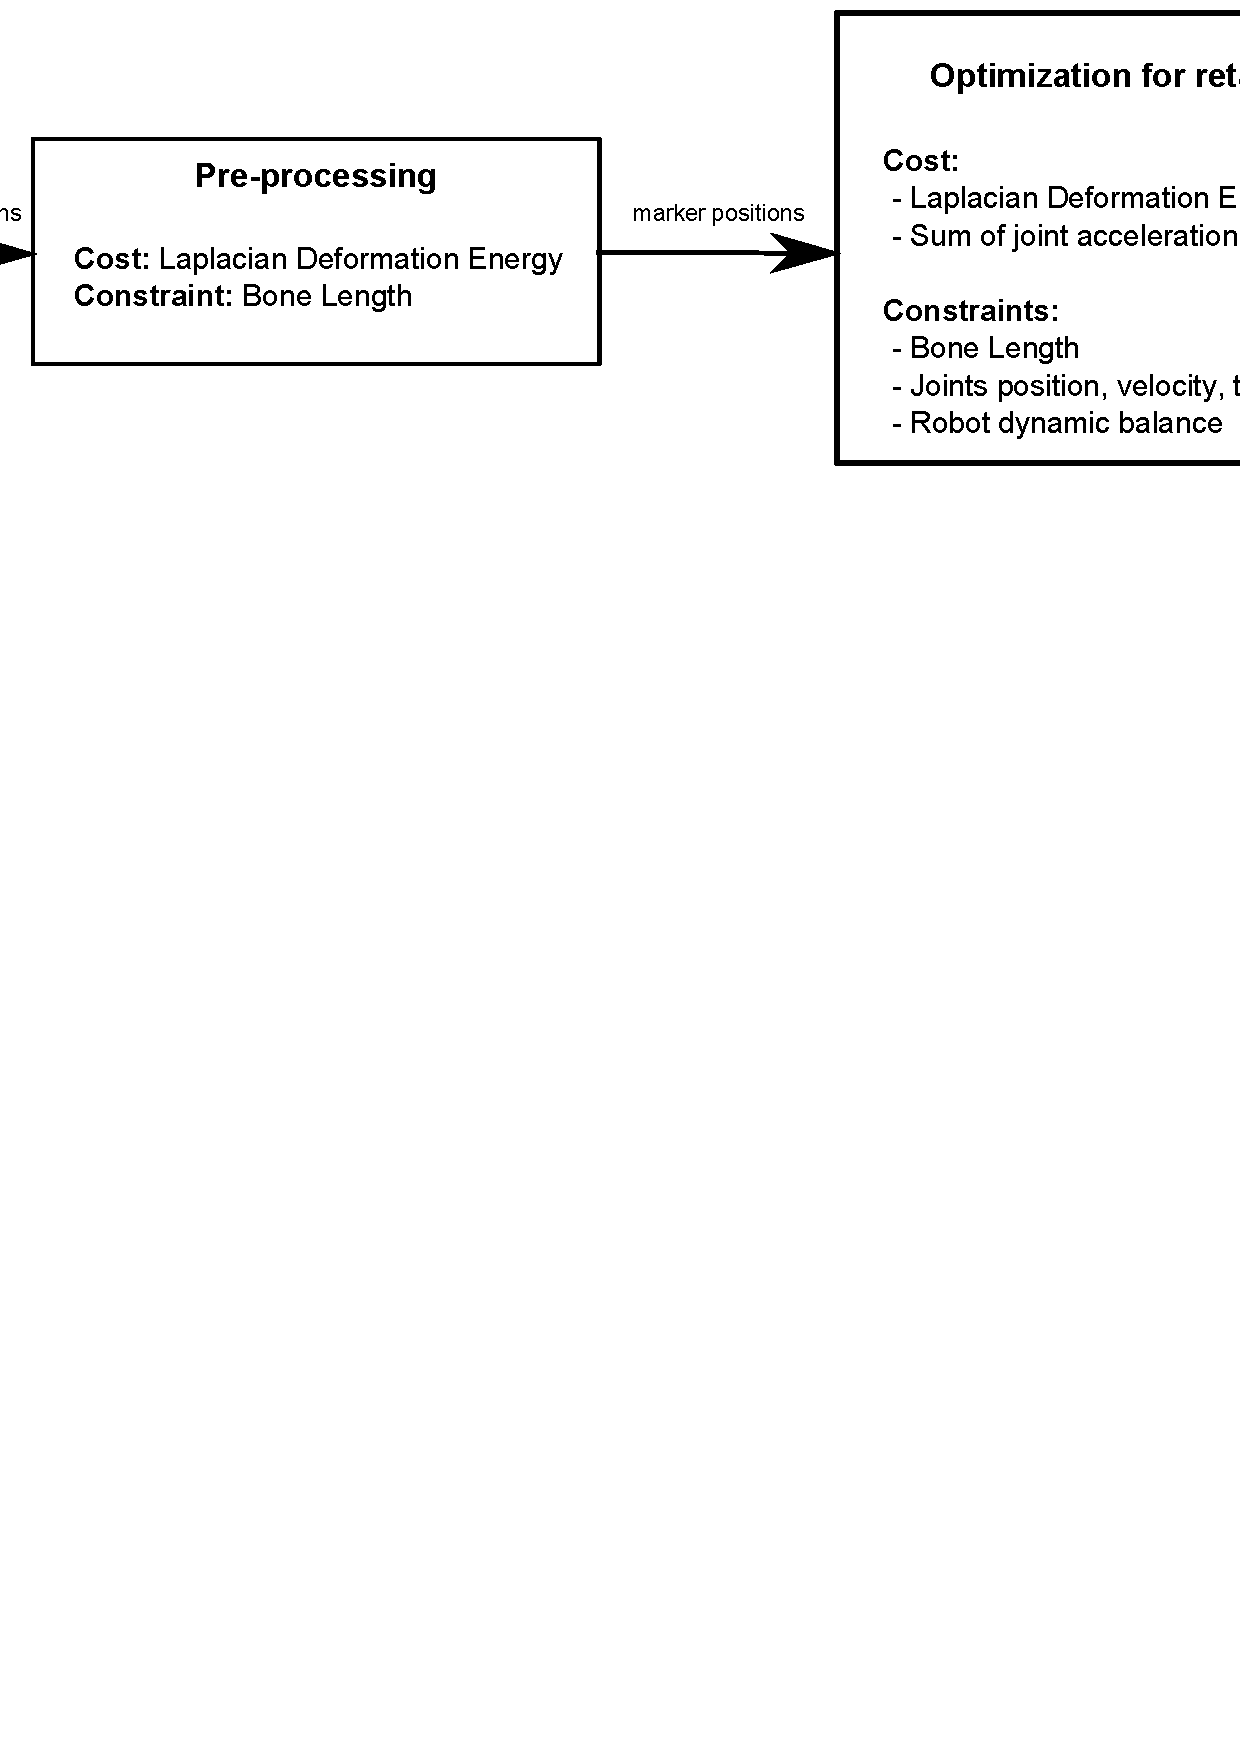
\includegraphics[width=\linewidth]{figure/architecture.pdf}
  \label{fig:algorithm}
  \caption{The two step retargeting process. The final inverse
    kinematics step is only here to convert the final motion to joints
    trajectory.}
\end{figure*}


On the other hand, motion retargeting has been investigated
intensively in computer graphics domain, typically to generate motions
for new characters based on motion capture data using space-time
constraints solver \cite{Gleicher98}.  Recently, Ho et al\. proposed a
new retargeting method called ``interaction mesh'' that preserves the
spatial relationship between closely interacting body parts and
objects in the environments \cite{Komura10}.  Nakaoka and Kokura
extended this method for retargeting to a humanoid robot by taking
advantage of its capacity to adapt motions to a character with highly
different physical properties \cite{Nakaoka12Humanoids}. Usage of
interaction mesh brings natural following of original human motion and
self-collision avoidance.  Although this method includes quasi-static
balance consideration by shifting the waist, it does not deal with
dynamic constraints such as torque limits or dynamic ZMP-based
stability. In addition, those constraints are treated separately after
generating retargeted motion to adapt to the humanoid.


% Optim
Another related domain is the optimization technique that is more and
more employed to generate robot trajectories minimizing certain cost
function under mechanical or dynamic constraints. Miossec et
al\. applied nonlinear optimization dynamic whole-body motion like a
kicking motion of a human-size humanoid \cite{Miossec06ROBIO}.
Recently the optimization is utilized for generation of multi-contact
dynamic motion through modeling of dynamic constraints using Taylor
expansion \cite{Lengagne13IJRR}. Suleiman et al\. proposed another
trajectory optimization technique based on Lie algebra that allows
efficient computation through analytic integration of dynamics
\cite{Suleiman07Humanoids} and applied it to human motion imitation
\cite{Suleiman08ICRA}.  The latter research aims at optimizing the
humanoid trajectory to be as close as human motion, but self-collision
avoidance is incorporated as a post-processing to the optimized motion
like previous work \cite{Nakaoka12Humanoids}. This is disadvantageous
because separate application of collision avoidance may lead to
unnatural motions.



% Motivation and contributions
% Problem: dynamic constraints not well considered
% To our knowledge, there has been no motion optimization integrating
% motion retargeting and self-collision or interaction with
% environment at the same time.
Methods in previous research are, therefore, still lacking the
capability to optimize humanoid motions by taking into account
the associated problems for retargeting in a unified manner.
The main contribution of the paper is the optimization process
integrating retargeting, dynamics constraints and self-collision at
the same time, 
in order to create the humanoid motion as close to human motions as
possible. 
In this paper, we address this retargeting by formulating it
as a nonlinear optimization problem under spatial and dynamic
constraints.
%Our contributions are...
% the introduction of a two steps optimization process allowing to
% adapt motion to any humanoid shaped robots. 
First, the captured motion is pre-processed to provide better initial
guess for the optimization.
% Once the link length are resized to match the targeted robot morphology, 
Then the full optimization problem is solved
considering the spatial relationship and dynamic robotic constraints
simultaneously.  
The spatial relationship between body parts of captured motion is
reserved by using interaction mesh as introduced by \cite{Komura10},
which achieves self-collision avoidance in consequence. 
% In contrast to previous work including post-processing of the 
% generated motion to enforce some additional properties like
% self-collision avoidance, the proposed method has 
% the advantage that the whole
% problem is considered during the optimization problem which
% ensures robotics constraints while preserving spatial relationships.


%The paper is organized as follows...
This paper is organized as follows. Section~\ref{sec:overview}
describes the overall method and in particular how the retargeting
are performed. Section~\ref{sec:retargeting} describes the
details of each step of the optimization-based retargeting method.
% problem representation, each step of our retarget
% two optimization problems are defined. 
Section~\ref{sec:implementation} introduces 
RobOptim, an optimization framework for robotics used to implement the
proposed method. Section~\ref{sec:results} presents the results of
retargeting with validation of dynamic simulations, before concluding
the paper.

\section{Method Overview}
\label{sec:overview}


The method consists in two consecutive optimization problem. The first
optimization problem is considering only the retargeting problem
without integrating any robotics consideration (motion balance or
torque constraints). This geometric problem can be represented as a
linear problem with a quadratic cost rendering its resolution
extremely efficient.

Once this problem is solved, the full problem is then taken into
consideration. This problem is initialized using the result of the
first optimization problem to ease the convergence. The second problem
incorporates robotics constraints such as motion balance and torque
constraints. These constraints being non-linear this optimization
problem is much more computationally intensive.



\section{Retargeting Method}
\label{sec:retargeting}

\subsection{Modeling}

Contrary to the approach introduced in FIXME, the two optimization
problems are considering marker position as the problem optimization
variables. In previous work, first the markers were optimized before
adapting the motion by optimizing joint angles. On the opposite in our
case, to preserve a global framework only the marker position is
optimized along the process. On the opposite, we rely on inverse
kinematics to estimate the nearest robot configuration at each point
of time. Therefore, the robotics constraints are evaluated for the
estimation of the robot configuration deduced from marker positions.


\subsection{Motion retargeting}


\begin{figure*}[htbp!]
  %\includegraphics[width=\linewidth]{figure/retargeting.jpg}
  \label{fig:retargeting}
  \caption{The marker set before (a) and after (b) the initial
    retargeting phase.}
\end{figure*}


The first optimization problem has been described extensively in
FIXME. It relies on the notion of ``interaction mesh'' to ensure that
spatial relationship between bodies is preserved.

By applying Delaunay Tetrahedralization \cite{FIXME} on the marker
set, one can generate a mesh which is parameterized by the marker
positions $\mathbf{V}_i = (\mathbf{p}^i_1 \cdots \mathbf{p}^i_m)$
where $1 \leq n \leq n$. $n$ denotes here the number of frame
composing the motion and $m$ the number of markers in each
frame. $\mathbf{p}^i_1$ represents the position of the first marker in
the $i$-th frame.

Given a particular interaction mesh, one can compute the ``Laplacian
Coordinate'' of one marker as follow:

\begin{equation}\label{eq:laplacian-coordinate}
L(p^i_j) = \mathbf{p}_i^j - \sum_{l \in N_j} w^j_l \mathbf{p}^i_l
\end{equation}

In \autoref{eq:laplacian-coordinate}, $N_j$ is the one-ring
neighborhood of marker $j$ in the interaction mesh and $w^j_l$ is the
weight of the marker $l$ when computing the Laplacian Coordinate of
marker $j$. This weight is inversely proportional to the distance
between $j$ and $l$.

Considering these two notions, it is possible to introduce the
``Laplacian Deformation Energy'' associated to a marker set which
serve as a cost function in this problem:

\begin{equation}
E_L(\mathbf{V'}_i) = \sum_j || L(\mathbf{p}^i_j) - L(\mathbf{p}^i_j{}') ||^2
\end{equation}

The Laplacian Deformation Energy is the square of the norm of the
difference between the Laplacian Coordinates of the original marker
set and the updated marker set $\mathbf{V}'_i = (\mathbf{p}^i_1 \cdots
\mathbf{p}^i_m)$.

In practice, this cost function penalizes motion of highly-connected
markers whereas isolated ones will move for a lower cost.

% Talk about acceleration penalty?

A second cost function is added to the first one to smooth the
motion. To achieve this goal, the marker set acceleration energy is
considered:

\begin{equation}
  E_A(\mathbf{V}_{i-1}', \mathbf{V}_{i}', \mathbf{V}_{i+1}') =
  \frac{1}{2} || \mathbf{V}_{i-1}' - 2 \mathbf{V}_{i}' + \mathbf{V}_{i+1}' ||^2
\end{equation}

$\mathbf{V}_{i-1}'$, $\mathbf{V}_{i}'$, $\mathbf{V}_{i+1}'$ being the
new marker set position for the frame $i - 1$, $i$ and $i +
1$. Acceleration energy is always null for first and last frame.

The final cost function $C$ is by consequence expressed by:

\begin{equation}
    C(\mathbf{V}_{i-1}', \mathbf{V}_{i}', \mathbf{V}_{i+1}') =
    E_L(\mathbf{V}_{i}') + E_A(\mathbf{V}_{i-1}', \mathbf{V}_{i}', \mathbf{V}_{i+1}')
\end{equation}


Additionally, a link length constraint is defined. This constraint
aims at retargeting the motion so that it fits the robot
morphology. It is defined as follow:

\begin{equation}
|| \mathbf{p}^1_e - \mathbf{p}^2_e ||^2 = l_e
\end{equation}


Whenever there is a need for some part of the robot body to stay
fixed, an optional positional constraint is also provided through an
equality constraint:

\begin{equation}
  \mathbf{V}_i' = \mathbf{P}_i
\end{equation}

With $0 \leq i \leq m$.

% FIXME: sparse matrices are used -> constraints and cost function
% jacobian mostly empty. See
% http://homepages.inf.ed.ac.uk/tkomura/SIGGRAPH10_preprint.pdf


The quadratic problem is then solved to generate a new set of marker
position. This set of marker position is now fitting the robot
structure but may still not being feasible due to physical
constraints. Therefore, this process is not enough to generate a
feasible robotics motion. The next section will show how to refine
this motion to ensure that physical constraints are respected.


\subsection{Robotics motion generation}


From the motion generated in the previous section, we will define a
second non-linear optimization problem. The second optimization
problem will use the same optimization variables than the first one,
the same cost function and the same link length and positional
constraints.


By keeping the previous constraints, one is making sure that the good
properties ensured by the previous phase are kept during this
optimization step.


However, to ensure that the motion is feasible, two additional
constraints are added:
\begin{itemize}
\item Dynamic balance constraint.
\item Joints position, velocity and torque constraints.
\end{itemize}


The first constraint constrains the ZMP position so that it stays into
the robot support polygon:

\begin{equation}
  \begin{array}{ccc}
    x_{ZMP} &=& x_G - \frac{\dot{\sigma}_y\ +\ m\ z_G\ \ddot{x}_G}{m\ (\ddot{z}_G + g)} \\
    y_{ZMP} &=& y_G + \frac{\dot{\sigma}_x\ -\ m\ z_G\ \ddot{y}_G}{m\ (\ddot{z}_G + g)}
    \end{array}
\end{equation}

Where $(x_{ZMP}, y_{ZMP})$ is the ZMP position on the
ground. $\dot{\sigma}$ the variation of the kinetic momentum around
the center of mass and $(x_G, y_G, z_G)$ the center of mass
position. $g$ is the gravitational constant.

The ZMP acts as a criterion allowing to decide whether a motion is
balanced or not. As long as it stays inside the convex hull of the
robot contact points, the motion is stable.

Knowing which sole of the robot is in contact with the floor and the
sole geometry, it is possible to insert this equation as a constraint
to make sure the ZMP is staying inside the current support polygon.


The second robotics constraint we take into account in this problem
are the joints limitations. Given $(\mathbf{q}, \dot{\mathbf{q}},
\ddot{\mathbf{q}})$, the inverse dynamics algorithm \cite{FIXME} will
compute $\mathbf{\tau} = (\tau_1, \cdots, \tau_o)$ the set of torques
applied to each robot joint using the classical equation of motion:

\begin{equation}
  \mathbf{M}(\mathbf{q}) \ddot{\mathbf{q}} + \mathbf{C}(\mathbf{q},
  \dot{\mathbf{q}}) + \mathbf{G}(\mathbf{q}) = \mathbf{\tau}
\end{equation}

Where $\mathbf{M}(\mathbf{q})$ is the system mass matrix,
$\mathbf{C}(\mathbf{q}, \dot{\mathbf{q}})$ is the vector of Coriolis
and centrifugal forces and $\mathbf{G}(\mathbf{q})$ the vector of
gravitational forces.

Therefore, other constraints are expressed as:

\begin{equation}
  \begin{array}{ccc}
    \mathbf{q}_{min} \leq \mathbf{q} \leq \mathbf{q}_{max} \\
    \mathbf{dq}_{min} \leq \dot{\mathbf{q}} \leq \mathbf{dq}_{max} \\
    \mathbf{\tau}_{min} \leq \mathbf{\tau} \leq \mathbf{\tau}_{max} \\
    \end{array}
\end{equation}



\section{Implementation of the optimization problem using RobOptim}
\label{sec:implementation}


RobOptim is a framework to ease the development and resolution of
optimization problems applied to robotics. It relies on a three layer
architecture: the core layer provides a way to define mathematical
function and their associated derivatives, the solver layer encapsulates
different State of the Art solver so that they can solve problems
defined using the representation proposed by the Core layer. To finish
the application layer contains dedicated mathematical functions which
can be embedded into different optimization problems. An overview of
the framework architecture is \autoref{fig:roboptim}.


The interest of adopting such a framework is to take advantage of
higher level tools such as numerical differentiation, which can be
used when no analytical gradient is provided by the user. Even if the
gradient is provided, numerical differentiation can be used to ensure
the computation correctness.


\begin{figure}[htbp!]
  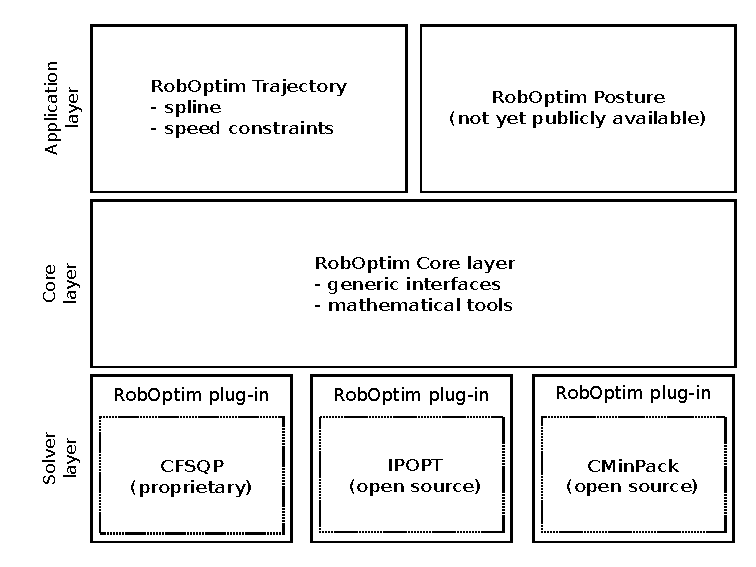
\includegraphics[width=\linewidth]{figure/roboptim-architecture.pdf}
  \label{fig:roboptim}
  \caption{RobOptim  architecture.}
\end{figure}


RobOptim is distributed as an open-source library (\mbox{LGPL-3}) through its
website: \url{http://www.roboptim.net/}



\section{Results and simulation}
\label{sec:results}


\begin{figure*}[htbp!]
  %\includegraphics[width=\linewidth]{figure/.pdf}
  FIXME FIXME FIXME
  \label{fig:results-torque}
  \caption{Joint torque after the first and second optimization
    phase.}
\end{figure*}



The proposed algorithm has been applied to different reaching and
grasping motion.


FIXME: list tested motion, draw graphs, make comparison.


These motions have been validated in a dynamic simulator to check for
balance issues. Dynamic simulation and visualization is provided by
the Choreonoid\footnote{\url{http://www.choreonoid.org/en/}} robotics
environment.



\section{Conclusion}
\label{sec:conclusion}

This paper presented a novel approach combining retargeting and
robotics constraints into one single nonlinear optimization
problem. To enhance convergence speed, an initial process solving only
the geometrical part of the problem as a quadratic problem. This
two-step approach has been validated through the use of a dynamics
simulator.

Future work includes taking into account additional constraints such
as auto-collision. Application to walking motion retargeting is also
considered.

% \addtolength{\textheight}{-12cm}   % This command serves to balance the column lengths
                                  % on the last page of the document manually. It shortens
                                  % the textheight of the last page by a suitable amount.
                                  % This command does not take effect until the next page
                                  % so it should come on the page before the last. Make
                                  % sure that you do not shorten the textheight too much.

%%%%%%%%%%%%%%%%%%%%%%%%%%%%%%%%%%%%%%%%%%%%%%%%%%%%%%%%%%%%%%%%%%%%%%%%%%%%%%%%



%%%%%%%%%%%%%%%%%%%%%%%%%%%%%%%%%%%%%%%%%%%%%%%%%%%%%%%%%%%%%%%%%%%%%%%%%%%%%%%%



%%%%%%%%%%%%%%%%%%%%%%%%%%%%%%%%%%%%%%%%%%%%%%%%%%%%%%%%%%%%%%%%%%%%%%%%%%%%%%%%
%\section*{Appendix}
%
%Appendixes should appear before the acknowledgment.
%
\section*{Acknowledgment}

This research was partially supported by the Japan Society for the
Promotion of Science (JSPS; Grant-in-Aid for JSPS Fellows P12803).

%%%%%%%%%%%%%%%%%%%%%%%%%%%%%%%%%%%%%%%%%%%%%%%%%%%%%%%%%%%%%%%%%%%%%%%%%%%%%%%%


\bibliographystyle{IEEEtran}
\bibliography{./jrl-bib/yoshida-main,./jrl-bib/yoshida-ca,./jrl-bib/humanoid,./jrl-bib/assist,./jrl-bib/graphics,./jrl-bib/jrl}


\end{document}
